\begin{figure*}[t]
\centering
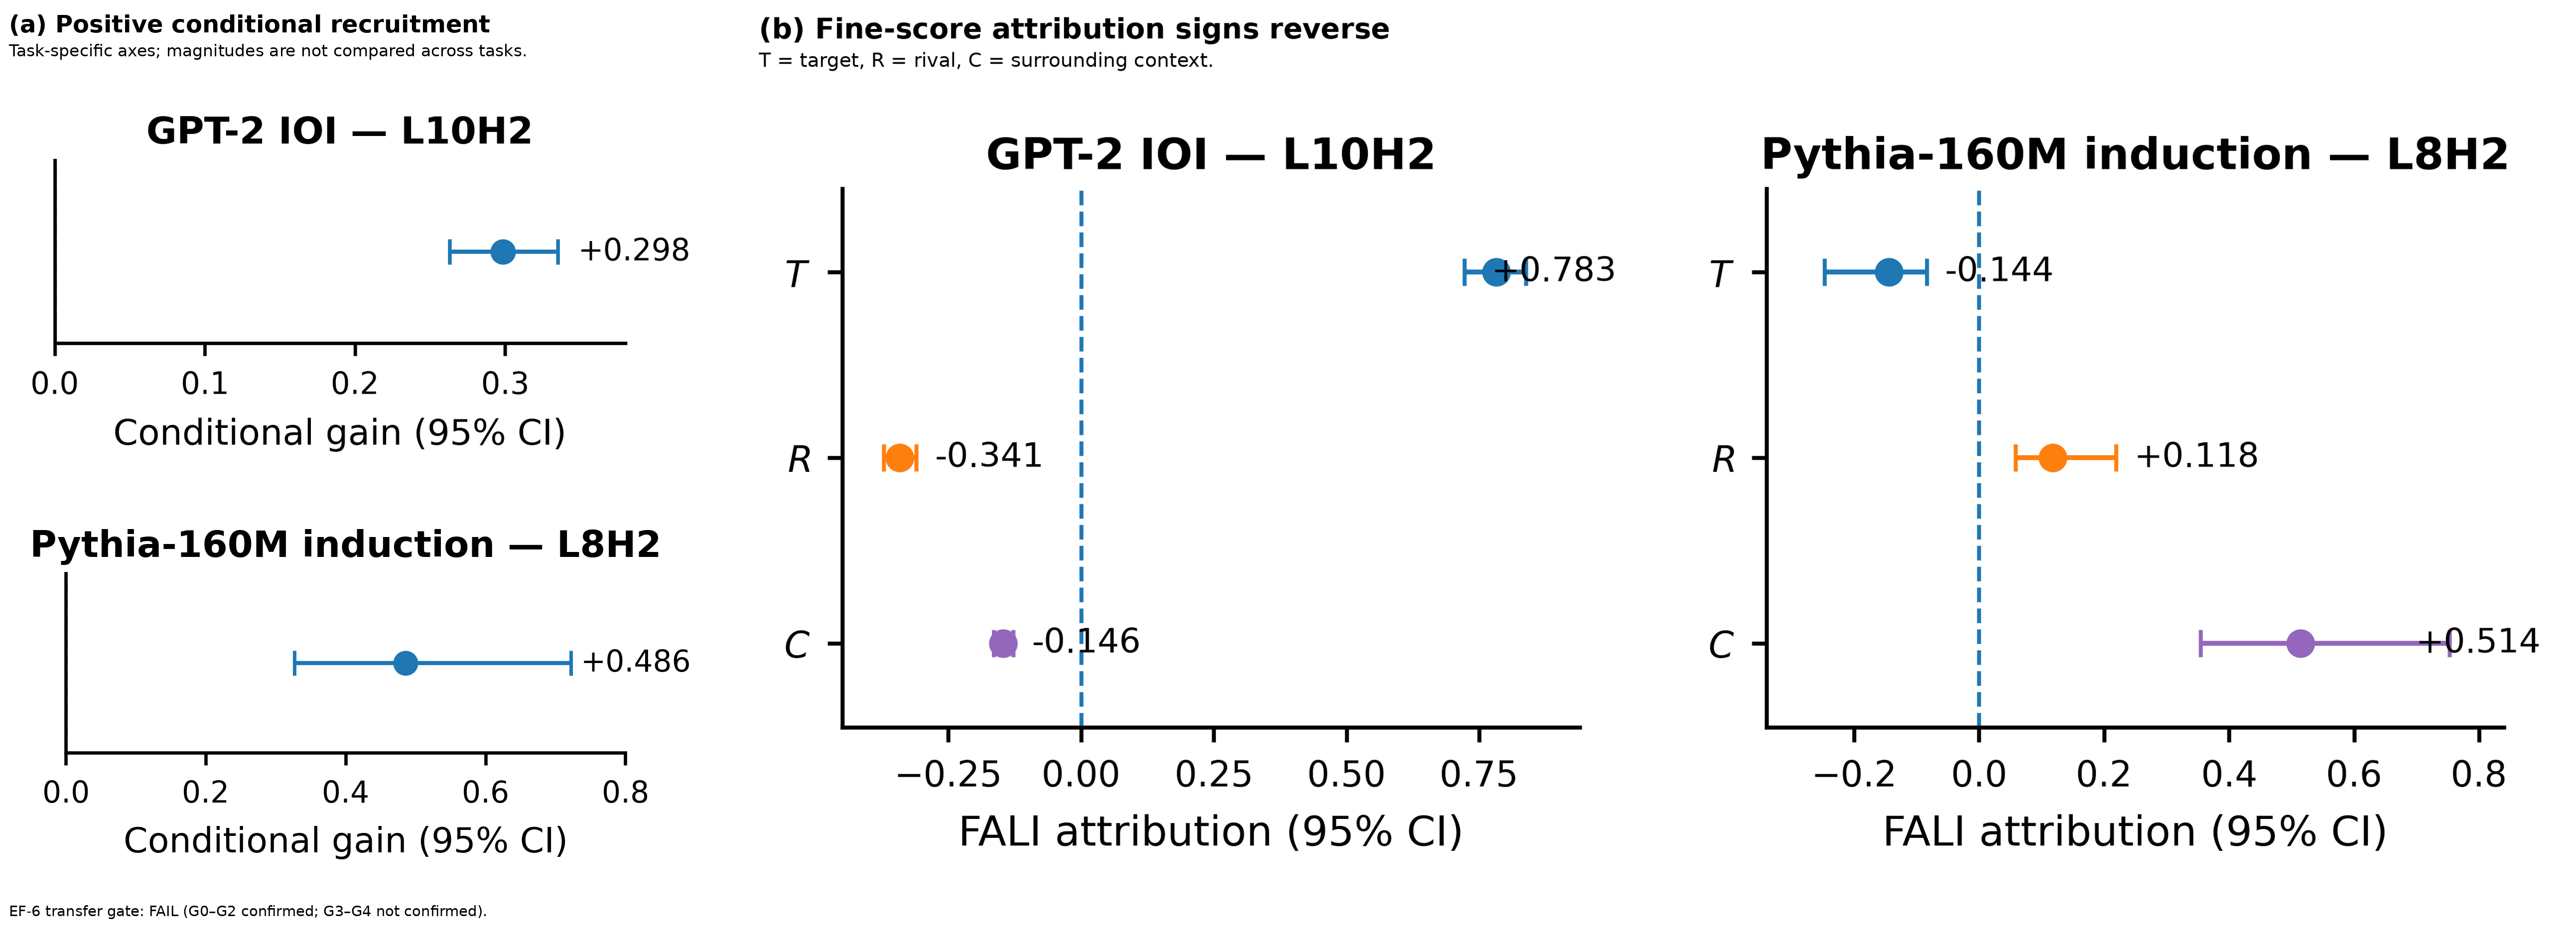
\includegraphics[width=\textwidth]{figures/Fig5.png}
\caption{\textbf{Conditional recruitment transfers across the two studied settings, but the preregistered fine-score mechanism does not.}
GPT-2 IOI L10H2 and Pythia-160M induction L8H2 both have positive conditional gain after their respective primary interventions; their raw attribution magnitudes are shown on task-specific utility scales and should not be compared directly.
Their fine FALI signs reverse: GPT-2 is target-positive/rival-negative with a negative context contribution, whereas Pythia is target-negative/rival-positive with a positive context contribution.
The preregistered Pythia transfer test therefore fails both sign-transfer gates while retaining confirmed induction behavior, primary-head importance, and conditional recruitment (G0--G2), giving an overall EF-6 transfer-gate failure.
Thus, a common functional recruitment response does not imply a common fine-grained mechanism.}
\label{fig:cross-setting-reversal}
\end{figure*}
